\documentclass[10pt,journal,compsoc]{IEEEtran}

\newcommand\MYhyperrefoptions{bookmarks=true,bookmarksnumbered=true,
pdfpagemode={UseOutlines},plainpages=false,pdfpagelabels=true,
colorlinks=true,linkcolor={black},citecolor={black},urlcolor={black},
pdftitle={Bare Demo of IEEEtran.cls for Computer Society Journals},%<!CHANGE!
pdfsubject={Typesetting},%<!CHANGE!
pdfauthor={Michael D. Shell},%<!CHANGE!
pdfkeywords={Computer Society, IEEEtran, journal, LaTeX, paper,
             template}}%<^!CHANGE!


\usepackage{graphicx}
\graphicspath{{res/}}
\usepackage{caption}
\usepackage{subcaption}

% correct bad hyphenation here
\hyphenation{op-tical net-works semi-conduc-tor}


\begin{document}

\title{Recognising people using body shape analysis}

\author{Man-Leong Chan,~\IEEEmembership{University of Southampton}}


\IEEEcompsocitemizethanks{\IEEEcompsocthanksitem M. Shell is with the Department
of Electrical and Computer Engineering, Georgia Institute of Technology, Atlanta,
GA, 30332.\protect\\
% note need leading \protect in front of \\ to get a newline within \thanks as
% \\ is fragile and will error, could use \hfil\break instead.
E-mail: see http://www.michaelshell.org/contact.html
\IEEEcompsocthanksitem J. Doe and J. Doe are with Anonymous University.}% <-this % stops a space
\thanks{Manuscript received April 19, 2005; revised December 27, 2012.}


% The paper headers
\markboth{Recognising people using body shape analysis, Biometric, May~2018}%
{Shell \MakeLowercase{\textit{et al.}}: Bare Advanced Demo of IEEEtran.cls for Journals}
\IEEEtitleabstractindextext{%
\begin{abstract}
The abstract goes here.
\end{abstract}

% Note that keywords are not normally used for peerreview papers.
\begin{IEEEkeywords}
Computer Society, IEEEtran, journal, \LaTeX, paper, template.
\end{IEEEkeywords}}


% make the title area
\maketitle
\IEEEdisplaynontitleabstractindextext
\IEEEpeerreviewmaketitle



\section{Introduction}



\IEEEPARstart{T}{his} demo file is intended to serve as a ``starter file''
for IEEE Computer Society journal papers produced under \LaTeX\ using
IEEEtran.cls version 1.8 and later.
% You must have at least 2 lines in the paragraph with the drop letter
% (should never be an issue)
I wish you the best of success.

\hfill mds
 
\hfill December 27, 2012

\subsection{Subsection Heading Here}
Subsection text here.

% needed in second column of first page if using \IEEEpubid
%\IEEEpubidadjcol

\subsubsection{Subsubsection Heading Here}
Subsubsection text here.




\section{Image processing}

\subsection{Green screen and background removal}
Our domain is a set of photos each with a subject in front of a green screen standing on a treadmill. Subject extraction requires the removal of the green screen as well as any background captured outside of the green screen area. Couple of samples of green screen color reveals the average screen color to be \textit{rgb(56, 175, 93)}. Image area beyond the green screen area is cropped to remove excess background area. 

\begin{figure}[!htb]
\begin{subfigure}[h]{0.3\linewidth}
    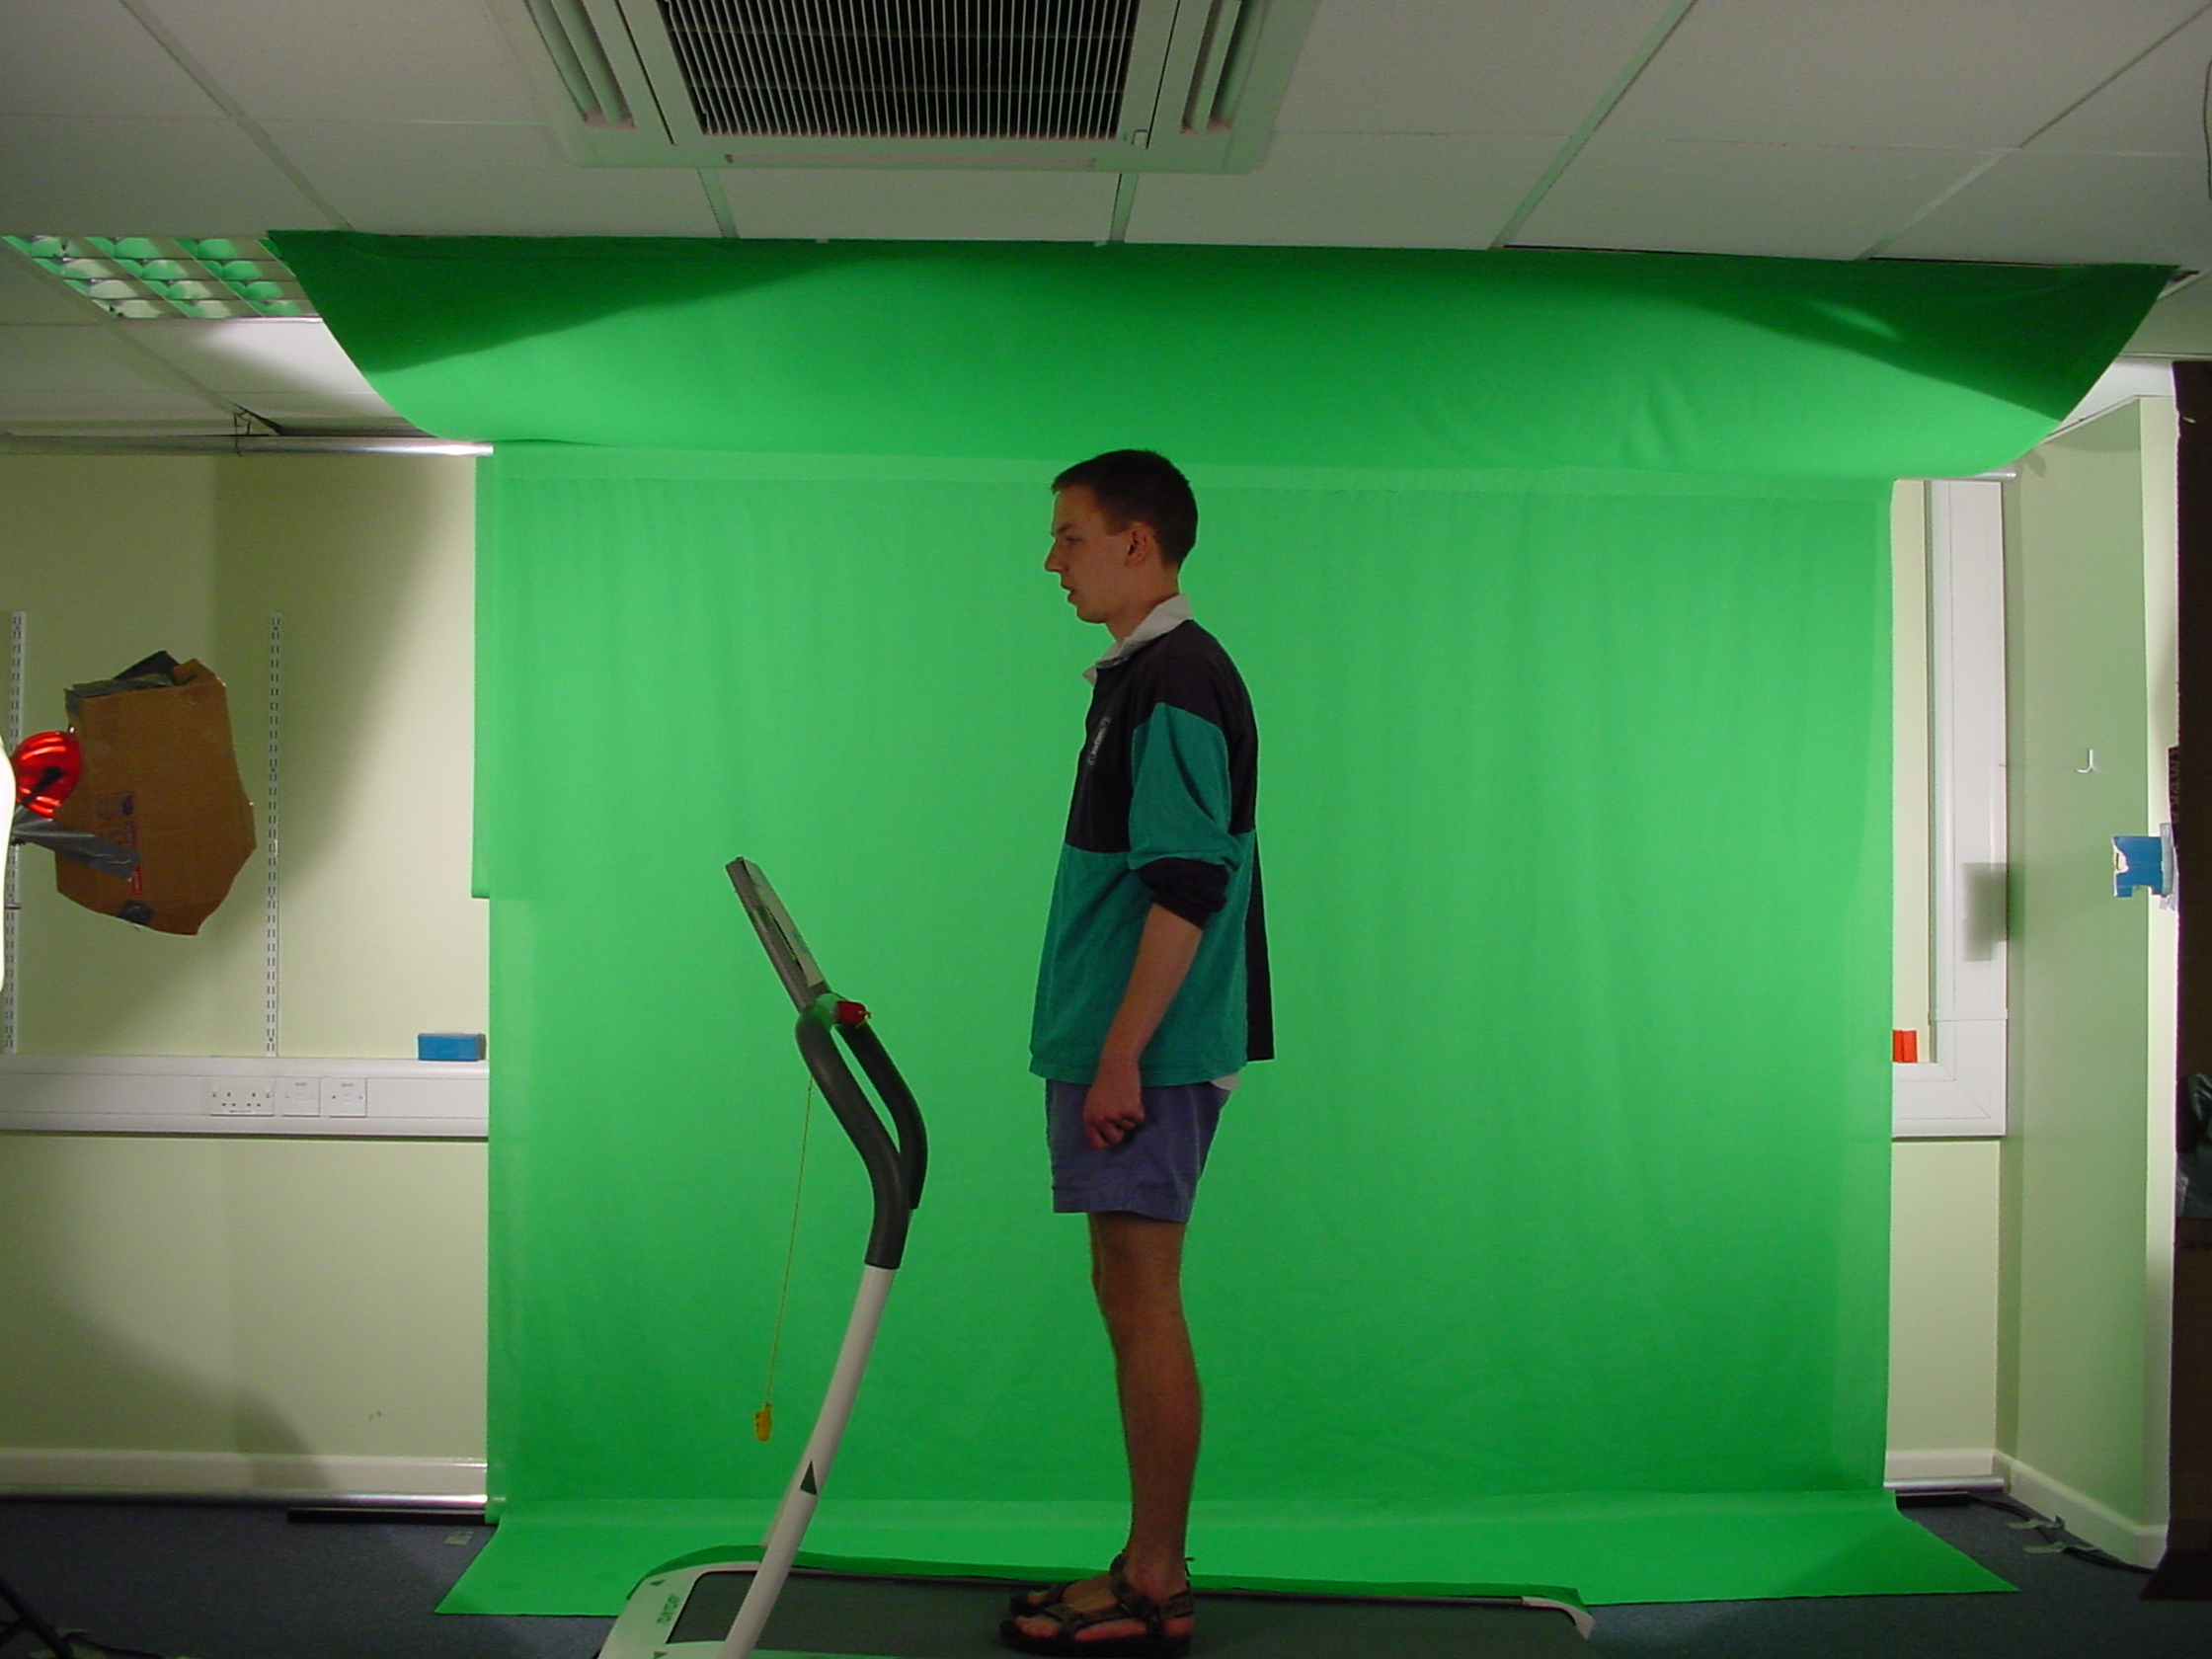
\includegraphics[width=\linewidth]{original}
\caption{Original}
\end{subfigure}
\hfill
\begin{subfigure}[h]{0.3\linewidth}
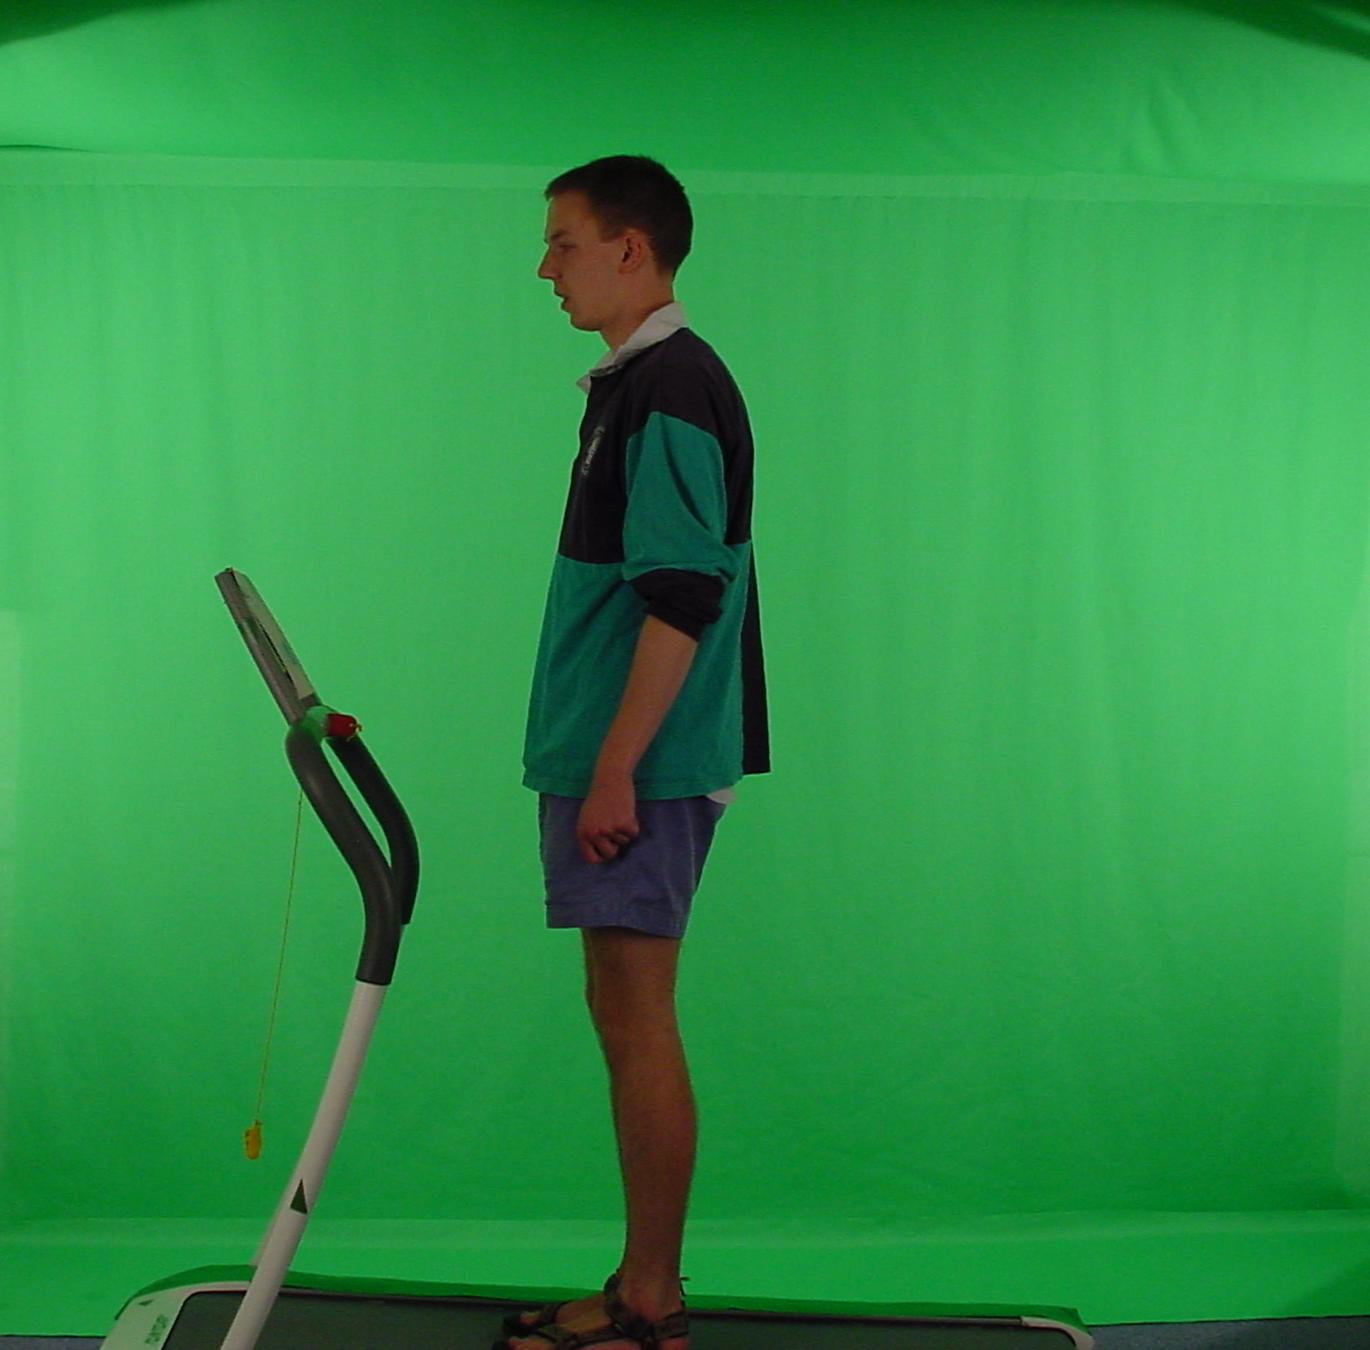
\includegraphics[width=\linewidth]{cropped}
\caption{Cropped}
\end{subfigure}
\hfill
\begin{subfigure}[h]{0.3\linewidth}
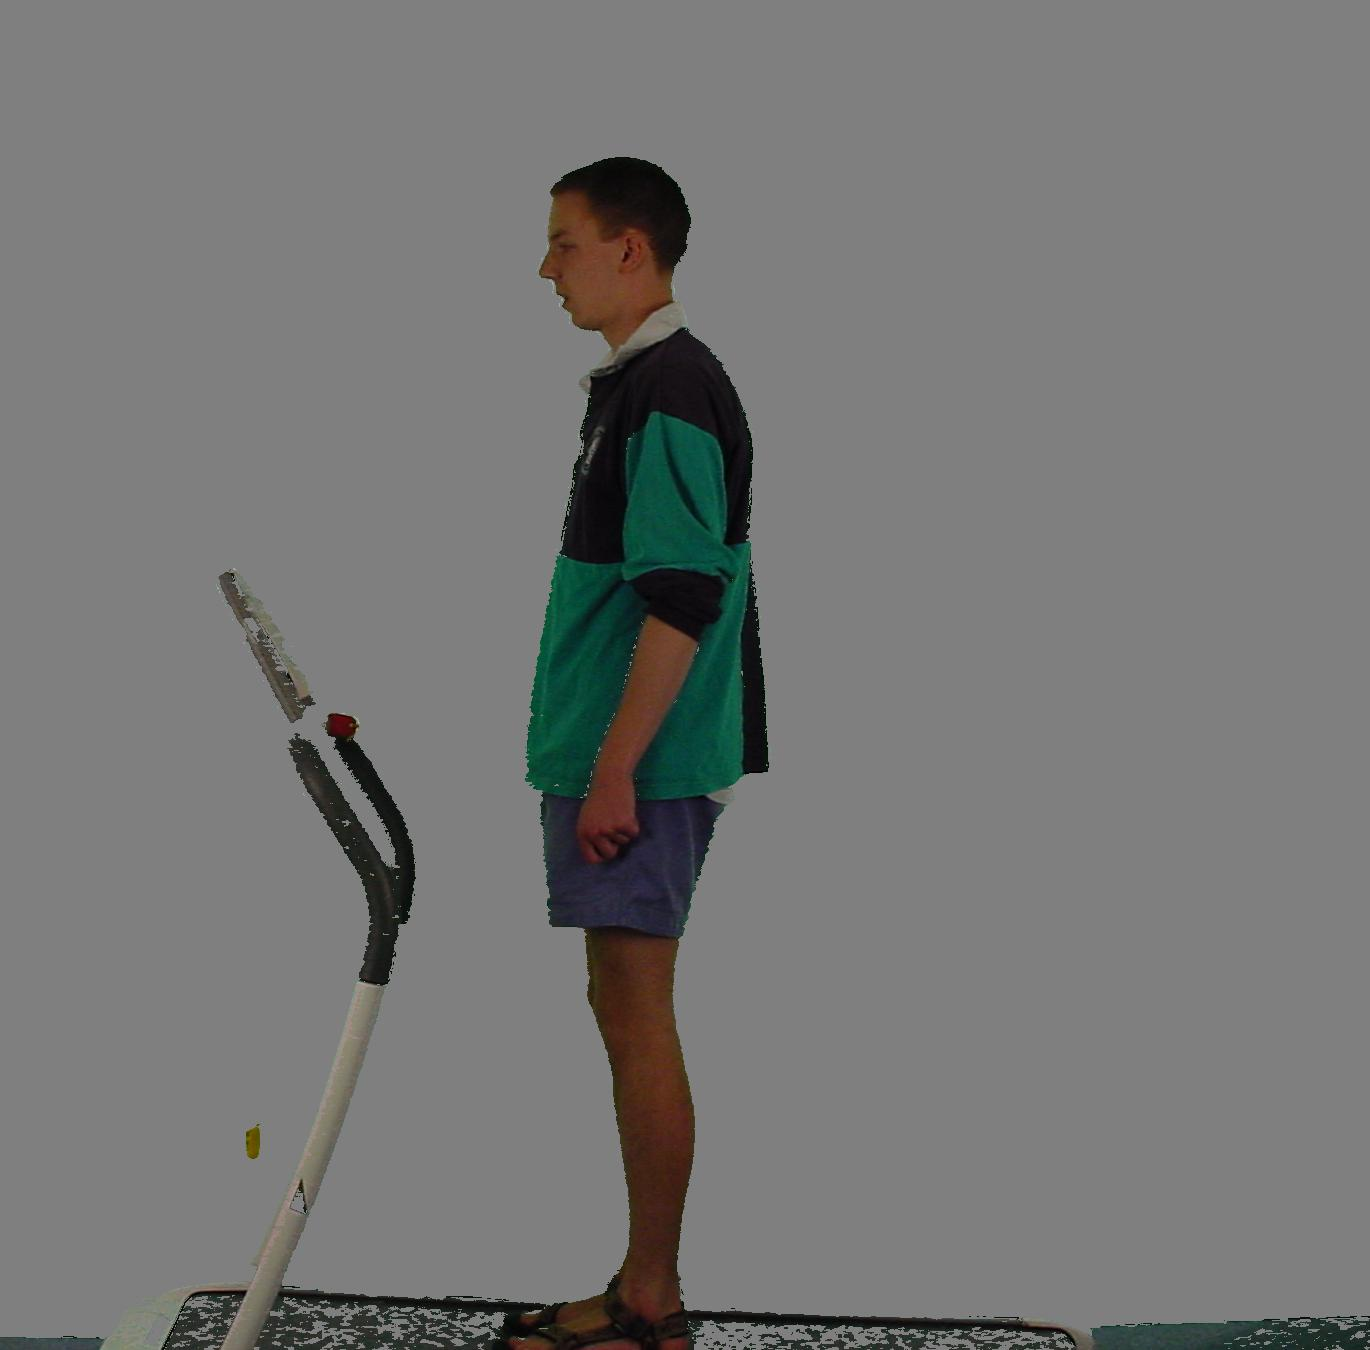
\includegraphics[width=\linewidth]{noGreen}
    \caption{bg removed}
\end{subfigure}%
\caption{Background removal}
\end{figure}


\subsection{Skin tone extraction}
Subject's limbs were extracted according to their skin tone. This extraction was done by analysing the HSV value of every pixel in the image. Where 0 \textless\textit{Hue} \textless25, 0.50 \textless\textit{Saturation} \textless0.98 and \textit{Value} \textgreater0.22. Our hue control selected skin tone from a range of color angles, it allowed the algorithm to be inclusive with a range of skin colour of different race and background. Saturation controled the range of colour sharpness which was crucial for our algorithm to differentiate between skin colour and shadows. The subject's skin surface under a reasonably well litted environment would have a higher saturation value than clothing in beige or brown.

\begin{figure}[!htb]
\begin{subfigure}[h]{0.45\linewidth}
    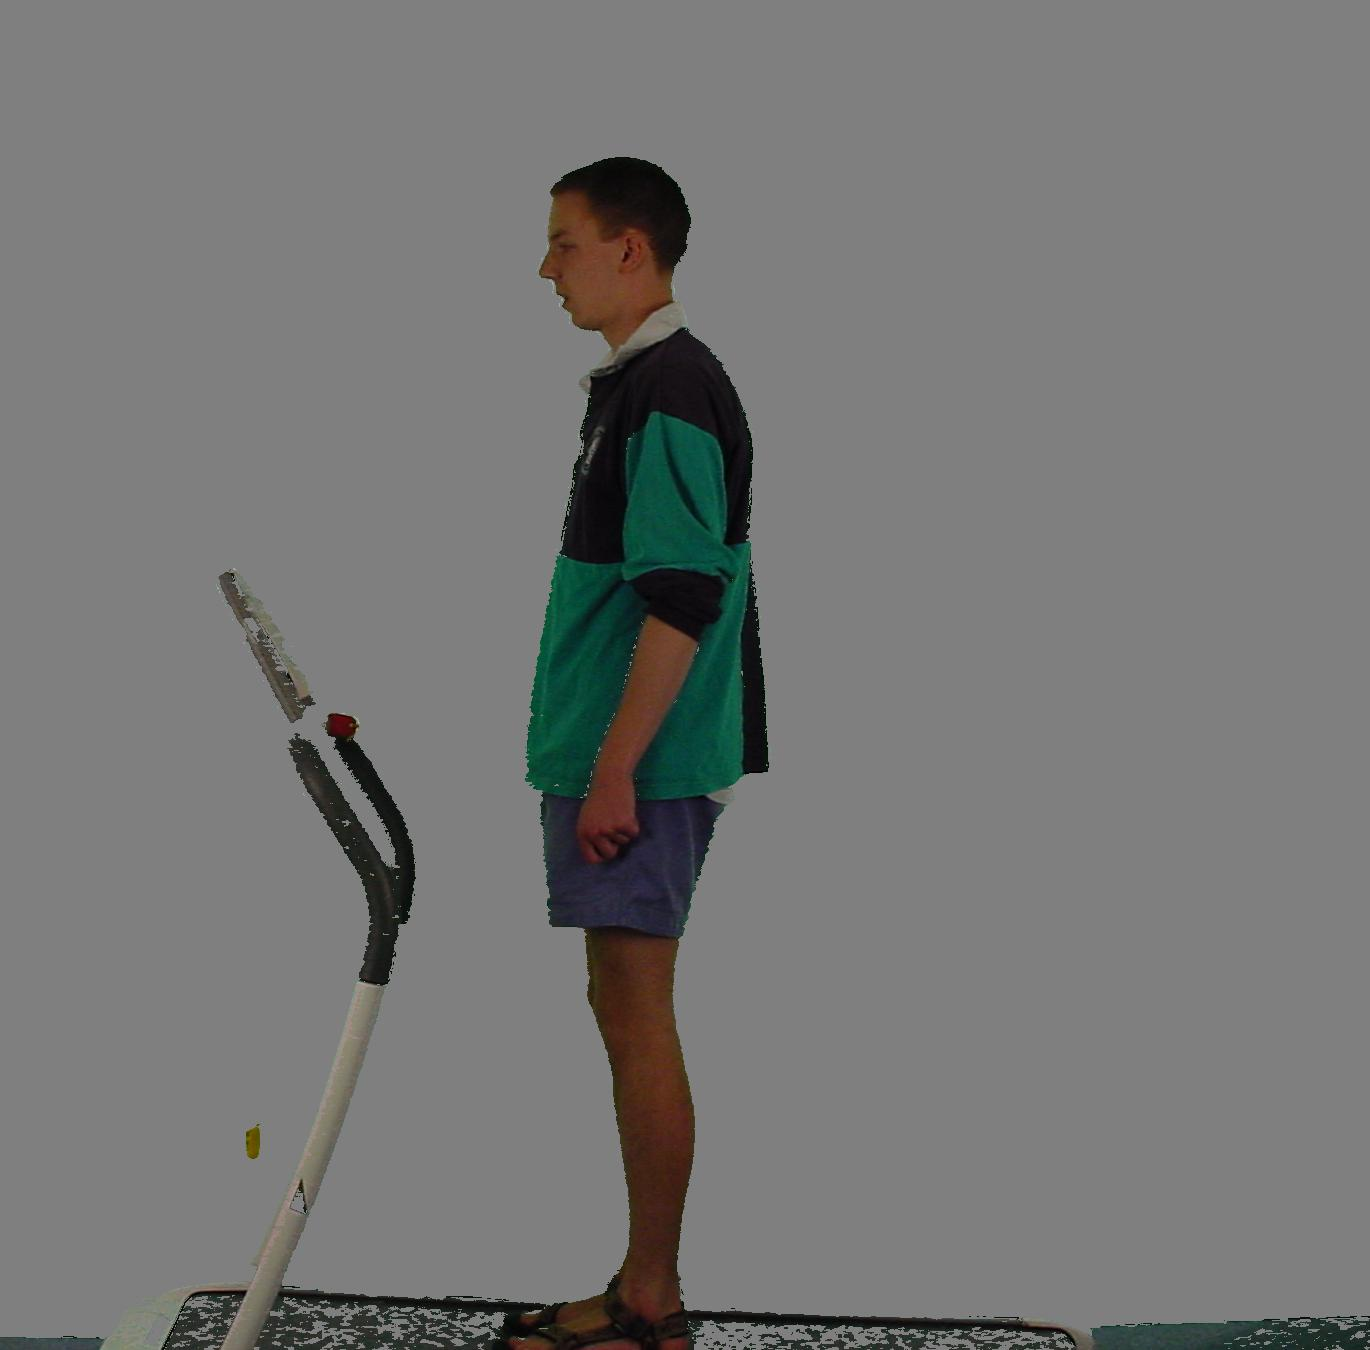
\includegraphics[width=\linewidth]{noGreen}
\caption{Before extraction}
\end{subfigure}
\hfill
\begin{subfigure}[h]{0.45\linewidth}
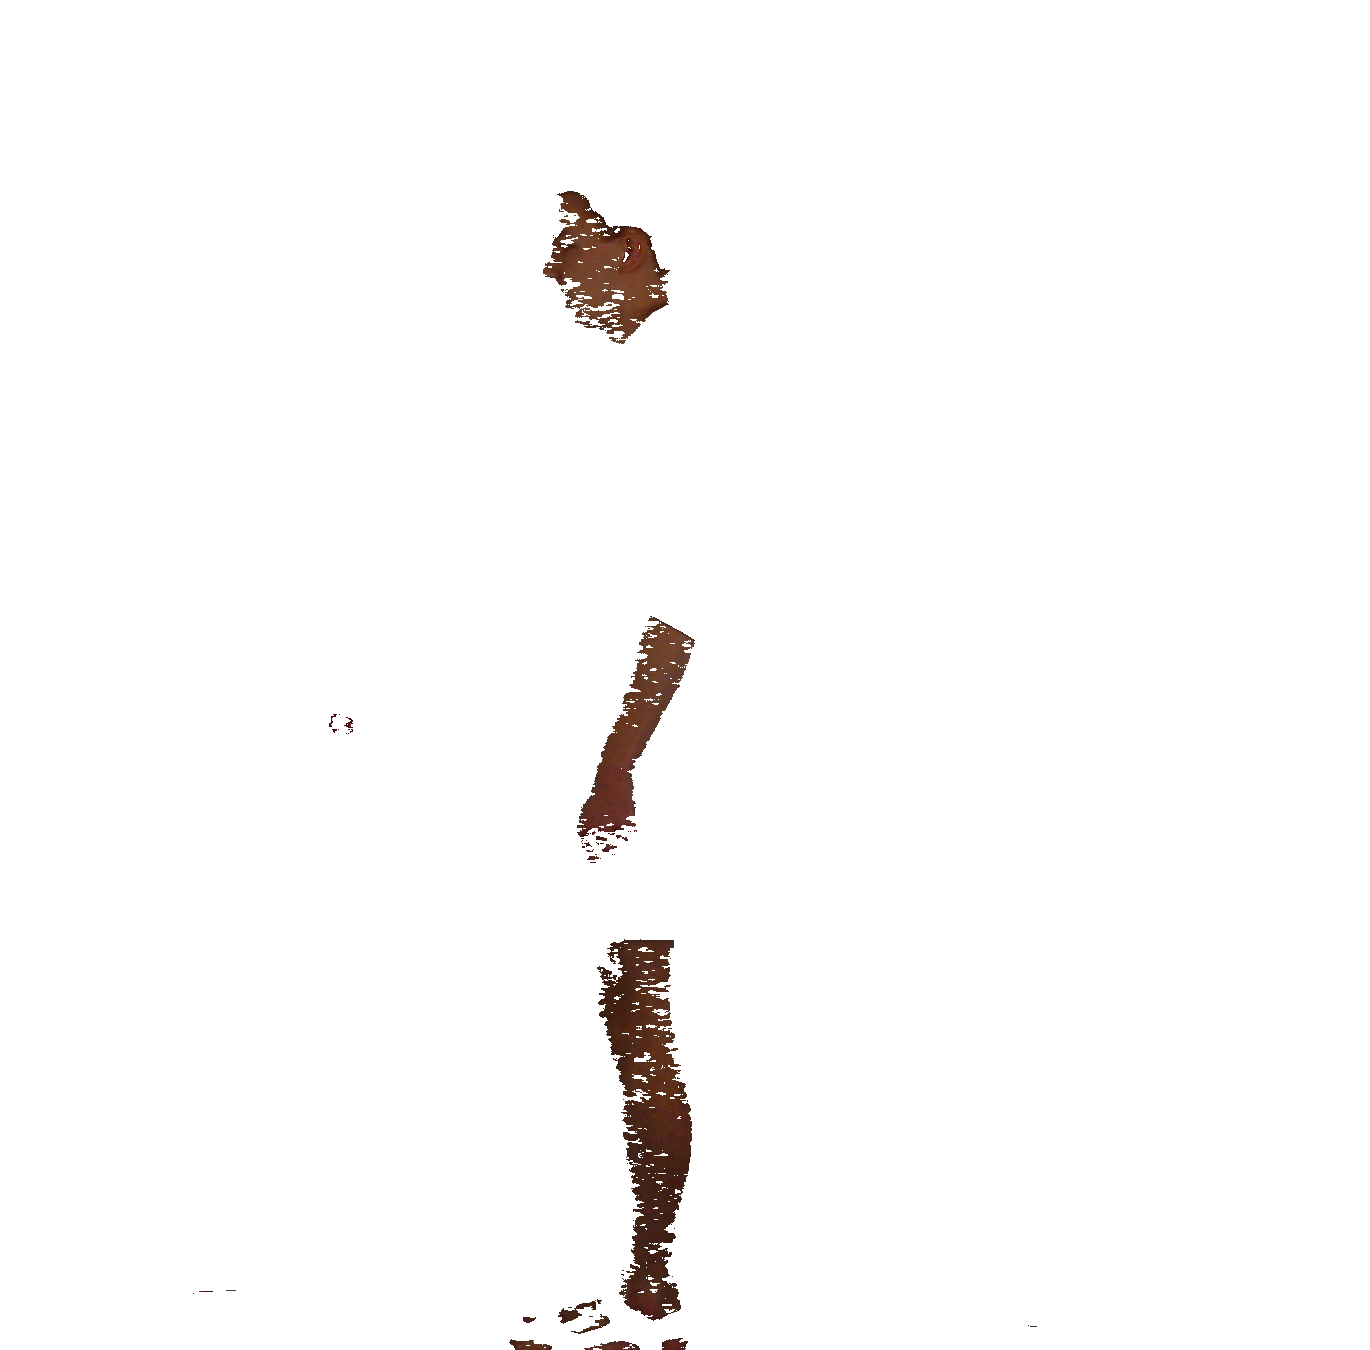
\includegraphics[width=\linewidth]{skin}
\caption{After extraction}
\end{subfigure}%
\caption{Skin tone extracton by HSV}
\end{figure}

Obviously tone extraction obviously relied on the subject exposing some part of their body. Primarily it required the subject to expose their face and hand for the best outcome. Therefore we are assuming that our subject does not wear a Niqab or gloves. 


\subsection{Limb Segmentation}
Skin tone extraction gave us many fragments of skin color in different sizes. The larger fragments gave us more interesting ideas on what those limbs could be, where as the smaller fragments scattered across the image could be noise which so happened to have the same HSV values as our subject's skin.
\\ \\
In order to carry out further analysis, we had to outline our desired fragments which were potentially part of subject's limbs. A floodfill analysis was used to determine the outline of those potential targets. It determined fragments which were connected in this 2 dimentional pixel array and output the outline of each fragments. Fragments which are smaller than any desired features were ignored to reduce noise in the data. 
\\ \\
Once the fragments were identified, they were subjected to feature analysis. Up to this point, the fragments are nothing but scattered data, feature analysis aims to identify which body part these fragments belong and this would give us useful data towards analysing subject's standing posture. Here we made a couple of assumption. 
\begin{itemize}
    \item Firstly the subject is not raising their hands above their head at the moment when the picture was taken. 
    \item Secondly the subject is not vertically rotated. 
\end{itemize}
Then we ran a verticle analysis where we first identify the person's head followed by their arms and leg. We assumed not everyone were wearing short and exposing the skin from their legs, so identifying legs were not compulsory. Similarly, some subjects were wearing long-sleeves and others were wearing t-shirts, the variation between the detected limb size were accounted for.


\begin{figure}[!htb]
\centering
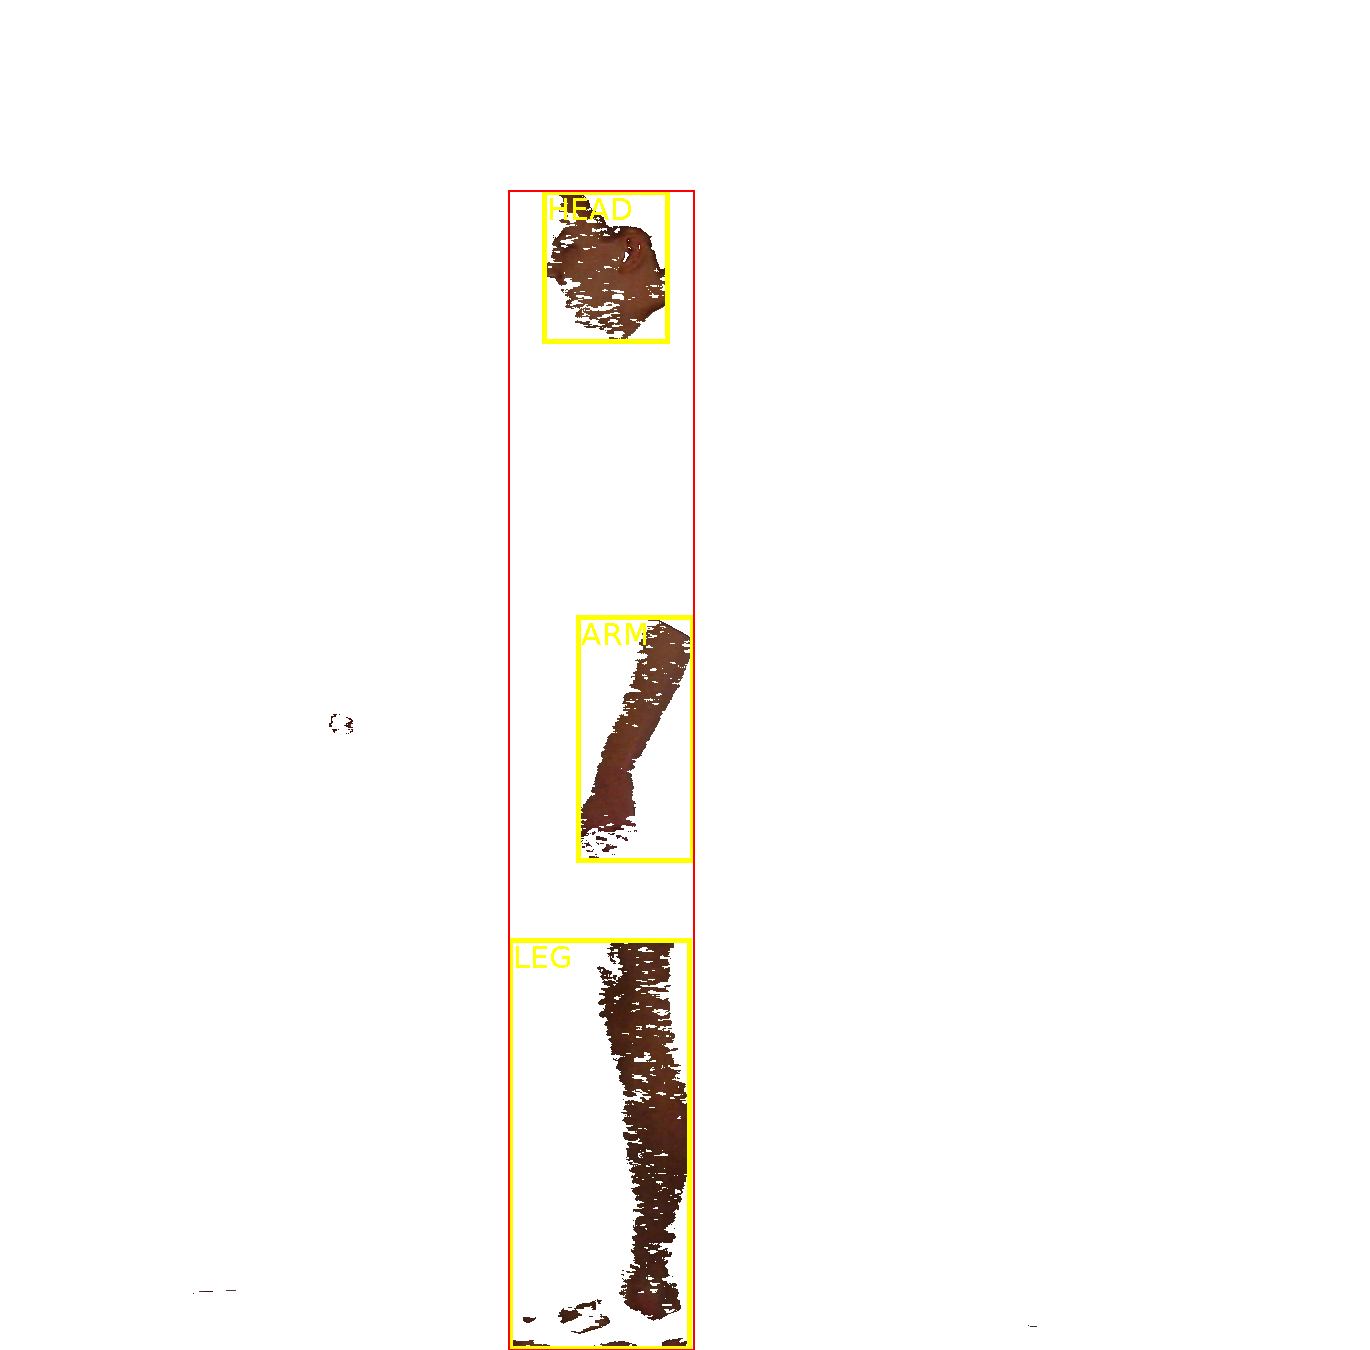
\includegraphics[width=0.7\linewidth]{segment_analysis}
\caption{Limb identification}
\end{figure}

\subsubsection{Statistics}
Accuracy of limb identification

\begin{center}
 \begin{tabular}{||l | l||} 
 \hline
 Total number of images &  112 \\ 
 \hline
 Number of limbs identified & 391 \\ 
 \hline
 False negatives & 8 \\
 \hline
 False positives & 25 \\
 \hline
 Error rate & 8.4\% \\
 \hline
\end{tabular}
\end{center}


\subsection{Silhouette extraction}
Edge detection technique was used to extract the subject's silhouette. All three common edge detection technique - Sobel, Roberts, Susan was tested ultimately Roberts' provided the cleanest results. Sobel gave us some vibrant lines but it contained too much redundent data of the treadmill.
\\ \\
The result of Roberts' were able to outline our subject and some of the treadmill. We used the parimeters of our limb segmentation to estimate our subject's location and ignored edges which were far away from the subject.

\begin{figure}[!htb]
\centering
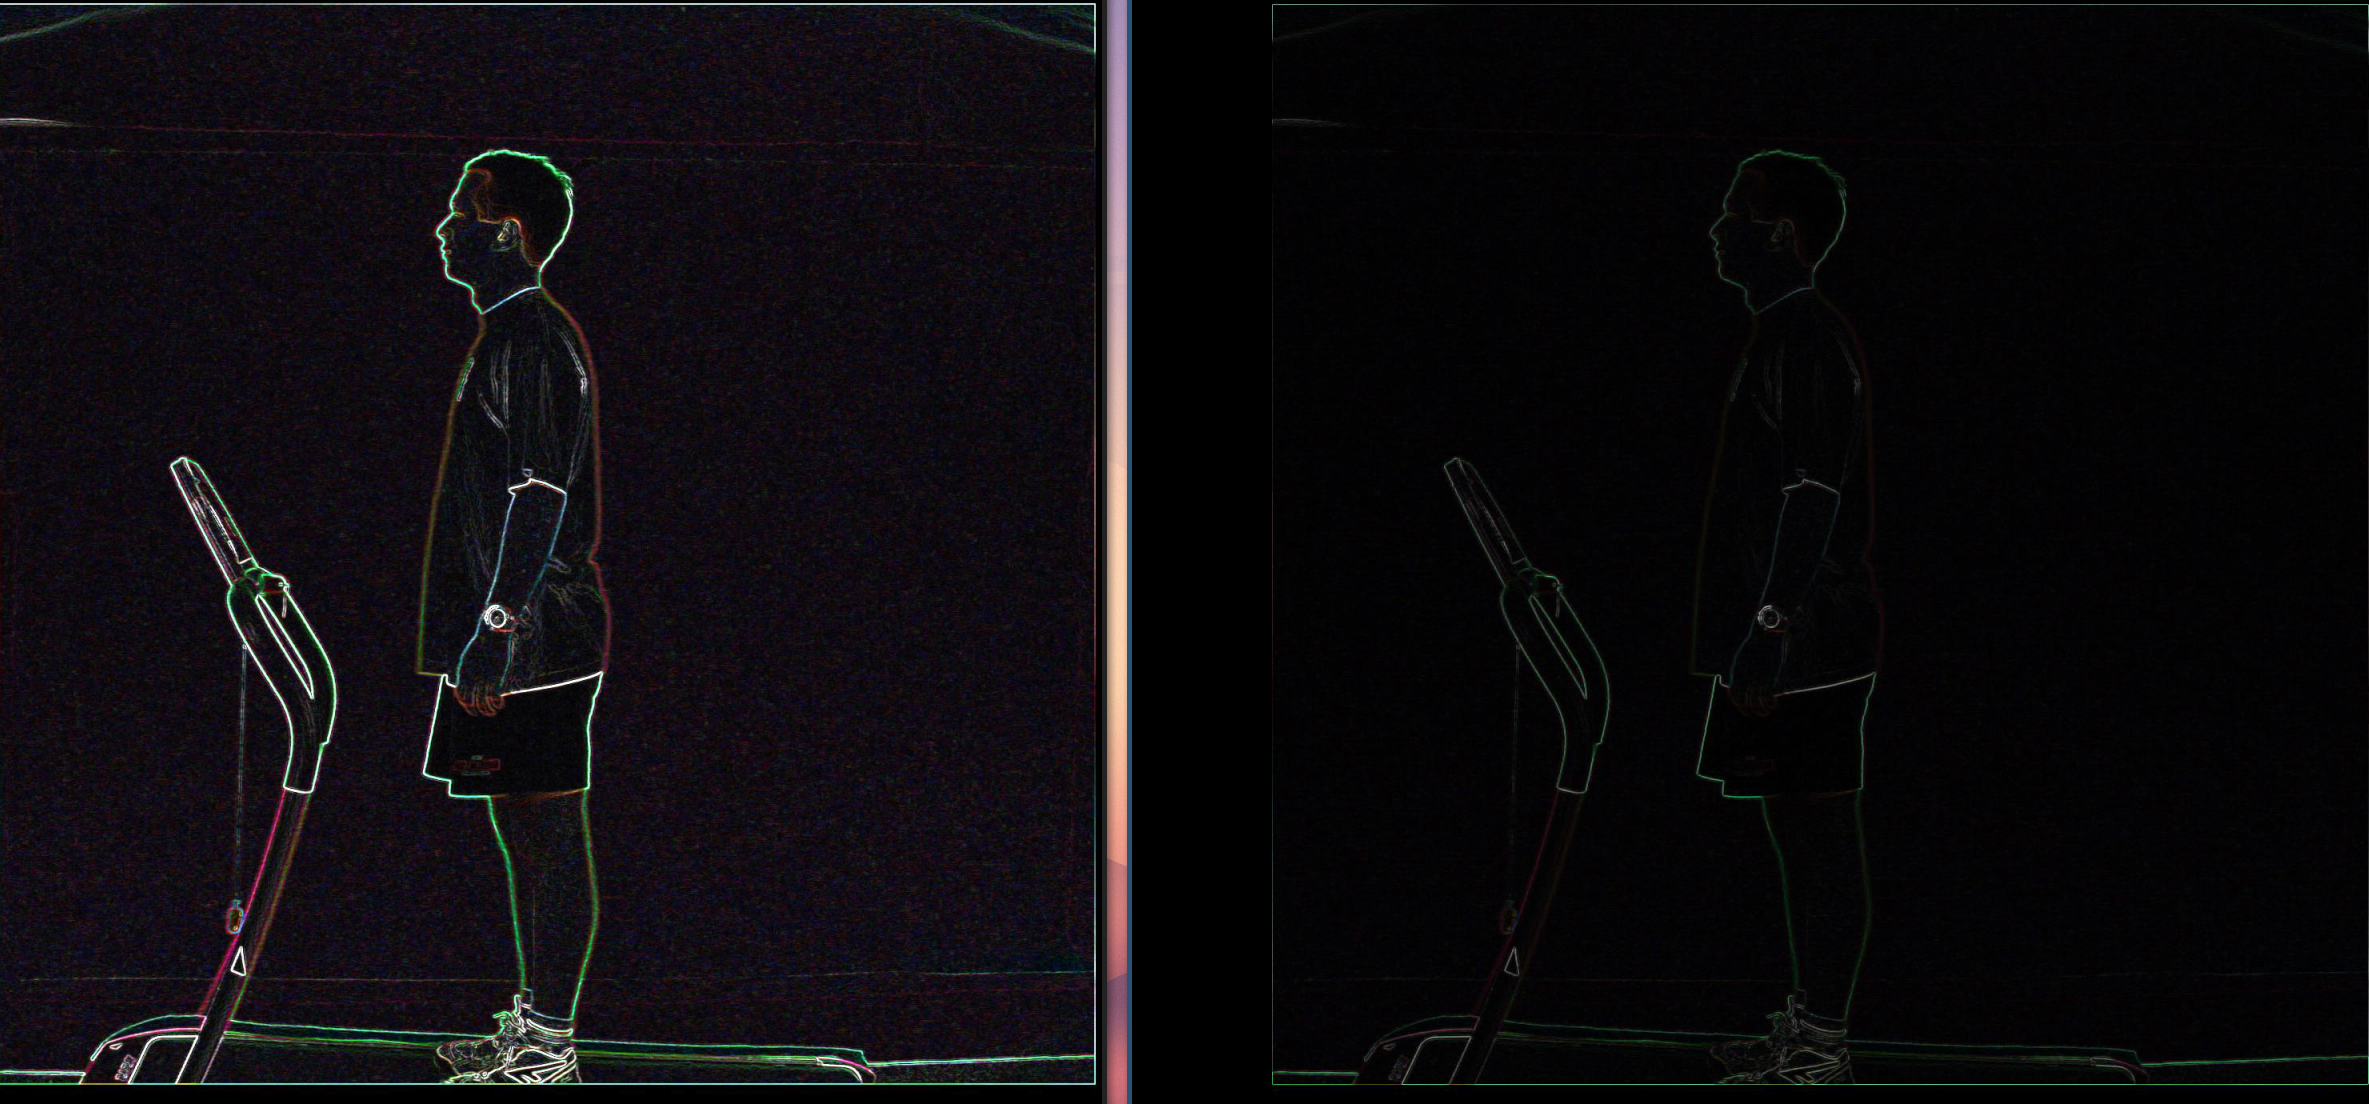
\includegraphics[width=0.7\linewidth]{edgeDetectionComp}
    \caption{Edge detection: Sobel (left) vs Roberts (right)}
\end{figure}

\subsection{Results}
The end result of both limb analysis and silhouette extraction has allowed us to gain a lot of metrics for further analysis into the subject's body shape as well as standing posture.

\begin{figure}[!htb]
\centering
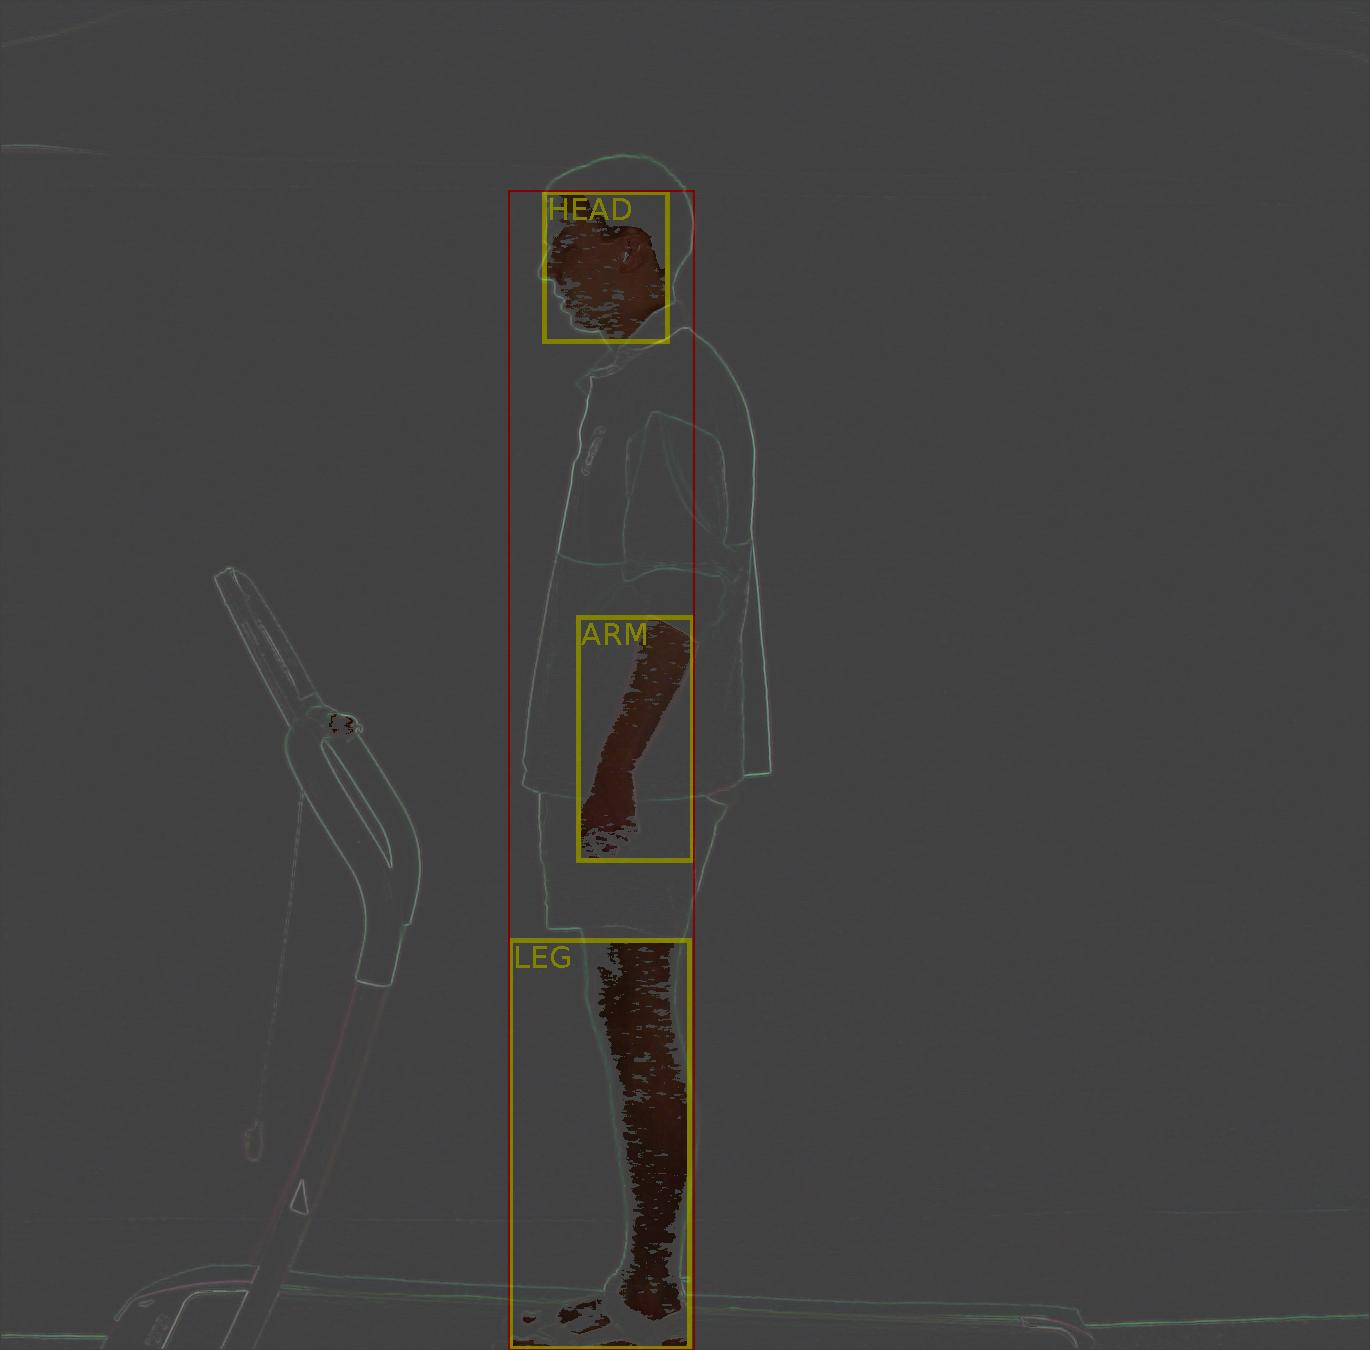
\includegraphics[width=0.7\linewidth]{combined}
    \caption{Silhouette with limb analysis}
\end{figure}



\section{Conclusion}
The conclusion goes here.


\appendices
\section{Proof of the First Zonklar Equation}
Appendix one text goes here.


\section{}
Appendix two text goes here.


% use section* for acknowledgement
\ifCLASSOPTIONcompsoc
  % The Computer Society usually uses the plural form
  \section*{Acknowledgments}
\else
  % regular IEEE prefers the singular form
  \section*{Acknowledgment}
\fi


The authors would like to thank


\ifCLASSOPTIONcaptionsoff
  \newpage
\fi

\begin{thebibliography}{1}

\bibitem{IEEEhowto:kopka}
H.~Kopka and P.~W. Daly, \emph{A Guide to {\LaTeX}}, 3rd~ed.\hskip 1em plus
  0.5em minus 0.4em\relax Harlow, England: Addison-Wesley, 1999.

\end{thebibliography}


\begin{IEEEbiography}{Michael Shell}
Biography text here.
\end{IEEEbiography}

% if you will not have a photo at all:
\begin{IEEEbiographynophoto}{John Doe}
Biography text here.
\end{IEEEbiographynophoto}

\begin{IEEEbiographynophoto}{Jane Doe}
Biography text here.
\end{IEEEbiographynophoto}

\end{document}



